\chapter{Usando \maggen}
\label{chap:usos}
\minitoc
Para usar \maggen\ debemos invocar la herramienta mediante la linea de comando, es decir, debemos contar con una terminal\footnote{En sistemas \textit{windows} compatible: win+R y luego \texttt{cmd} y en sistemas \textit{unix}: Alt+f2 y luego \texttt{xterm}} para su funcionamiento. Por cuestiones de simpicidad y flexibilidad de la herramienta, no se considero el desarrollo de un \textit{front-end} para \maggen. Además, debemos tener en cuenta, que el usuario presentara interes en el resultado generado de \maggen y no de una innecesaria interfaz grafica, que entorpeceria su comportamiento conbinatorio con otros comandos.
  
\maggen\ puede ser invocado utilizando una serie de parametros que inciden directamente sobre el resultados producido por la herramienta. En el desarrollo de este capitulo trataremos estos temas en detalles y ademas analizaremos el uso del evaluador generado por \maggen.

\section{Uso de \maggen: Parametros y opciones}
La totalidad de parámetros y opciones de \maggen\ son opcionales. La sintaxis de invocación de la herramienta esta dada por:\\
\begin{center}\texttt{maggen [OPTIONS]}\end{center}
Las opciones son las siguientes:
\begin{description}
\item [-f  file] Definir el archivo de entrada de \maggen\ como \texttt{file}. Si omitimos esta opción \maggen espera la entrada por la entrada estándar (cin) hasta leer el caracter EOF (end of file) \footnote{En sistemas unix el caracter EOF puede ser producido con Ctrl+D dentro de una consola de comandos.}.
\item [-i  header] Incluir \texttt{header} en la generación de código. Genera un \texttt{\#include ``header''} del archivo que referencia esa ruta. Dicha linea, \maggen la agrega al archivo generado.
\item [-fo folder] Define \texttt{folder} como el directorio de salida para \maggen. Si omitimos esta opción, \maggen\ usa el folder por defecto ``\textit{./out\_maggen/}''.
\item [-o  name] Define a \texttt{name} como el nombre de la clase y del archivo generado por \maggen. Si omitimos esta opción, \maggen\ usa por defecto el nombre ``\textbf{mag\_eval}''.
\item [-h] Muestra mensaje de ayuda.
\end{description}
A continuación observemos algunos ejemplo de invocación de \maggen.
\begin{itemize}
\item Si invocamos:\\ \texttt{./maggen -h} obtenemos el siguiente mensaje de ayuda:
\begin{center}
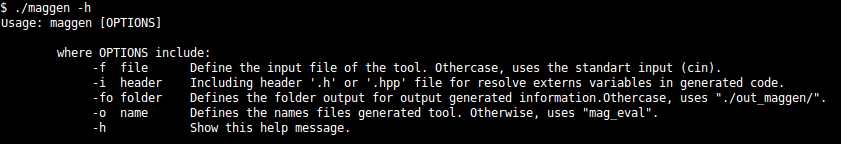
\includegraphics[width=350pt,height=60pt]{help.png}
\end{center}
\item Si invocamos: \\ \texttt{./maggen -fo ./Out\_wuu\_yang -o evalmag -f 
./examples/ag\_wuu\_yang/ag\_wuu\_yang.input}. \\ Especificamos como archivo de entrada a \texttt{ag\_wuu\_yang.input}, como directorio de salida \texttt{./Out\_wuu\_yang} y el nombre de la clase (y archivo) generada con el nombre \texttt{evalmag}. La figura \ref{fig:outnormal} muestra la salida de esta invocación.
\begin{figure}\centering
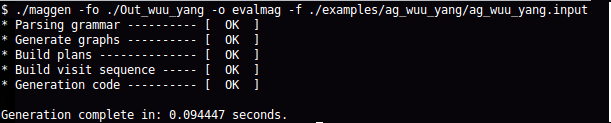
\includegraphics[width=350pt,height=70pt]{normal.png}
\caption{\label{fig:outnormal} Usando \maggen\ con opciones.}
\end{figure}

\item Si invocamos a \maggen\ sin la opción \texttt{-f} (independientemente que usemos o no las demas opciones) se espera la entrada por entrada estándar. Esto nos permite poder utilizar a \maggen\ en conjunto con otros comandos, Ejemplo:\\ \texttt{cat file | maggen -fo ./out/}.\\ 
Esto muestra a \maggen\ en conjunto con \texttt{cat} usando una tuberia (pipe o |).

\end{itemize}


 

\section{Uso del evaluador generado}
bla bla